\section{Higgs pair production} \label{sec:Higgs_Pair_Production}

A process through which the Higgs self-coupling can be directly accessed is Higgs pair production, the production of two Higgs bosons in a single process. The access of this coupling can allow for a measurement of its value, meaning that physics analyses of Higgs pair production can allow physicsts to provide experimental input into the shape of the Higgs potential. This comparison would be fundamental, and could have profound implications: This measurement may agree with the SM, or it may disagree and prompt physicists to consider how to reconcile the SM with their current observations. 

The two Feynman diagrams at leading order (LO) which have the largest impact on the production likelihood of Higgs pair production in the gluon-gluon fusion production mode are shown in Figure \ref{fig:HH_GF_LO_FD}.

\begin{figure}[H]% 
    \setcounter{subfigure}{0} % reset subcaption counter to 0 (a) 
    \centering
    \subfloat[Triangle diagram]{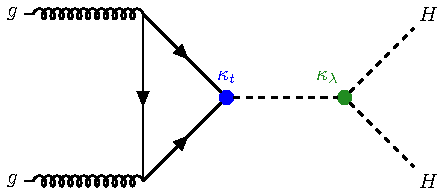
\includegraphics[width=.45\linewidth]{Images/Theory/fey_HH_Triangle.pdf}}%
    \qquad
    \subfloat[Box diagram]{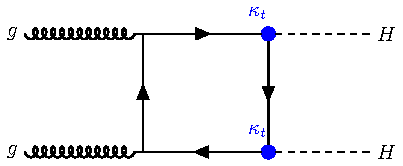
\includegraphics[width=.45\linewidth]{Images/Theory/fey_HH_Box.pdf}}%
    \caption{Leading order Higgs pair production Feynman diagrams in the gluon-gluon fusion production channel.}%
    \label{fig:HH_GF_LO_FD}
\end{figure}  

These diagrams are referred to as the ``triangle'' and ``box'' diagrams, where the triangle diagram is sensitive to both the Higgs self-coupling and top yukawa coupling (the coupling of the Higgs boson to two top quarks), while the box diagram is sensitive only to the top yukawa coupling. These diagrams destructively interfere in the computation of the process' matrix element, leading to a low production cross section. The contributions and interference of these two diagrams as a function of di-Higgs invariant mass for a center-of-mass energy of proton-proton collisions equal to $\sqrt{s} = 14 TeV$ is shown in Figure \ref{fig:LOXS_Contributions}. 

\begin{figure}[H]
    \centering
    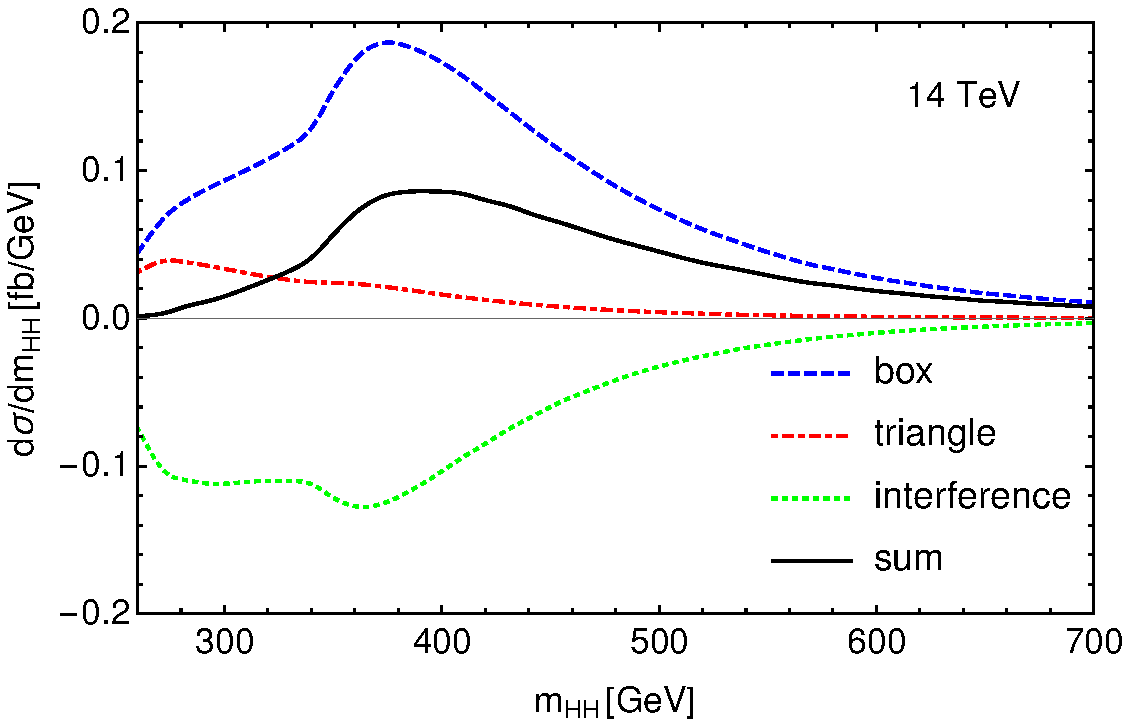
\includegraphics[width=0.85\textwidth]{Images/Theory/LO_contributions_ggF.pdf}
    \caption{Contribution to HH production cross section as a function of di-Higgs system invariant mass, for the triangle and box diagrams and their interference term.}
    \label{fig:LOXS_Contributions}
\end{figure}

Taking the higher order Feynman diagrams into account, including at next to leading order (NLO) and next-to-next-to leading order (NNLO), a more precise value of the di-Higgs production cross section is computed as a function of center of mass energy for different production modes, and is shown in Figure \ref{fig:ProductionModeXSs}. 

\begin{figure}[H]
    \centering
    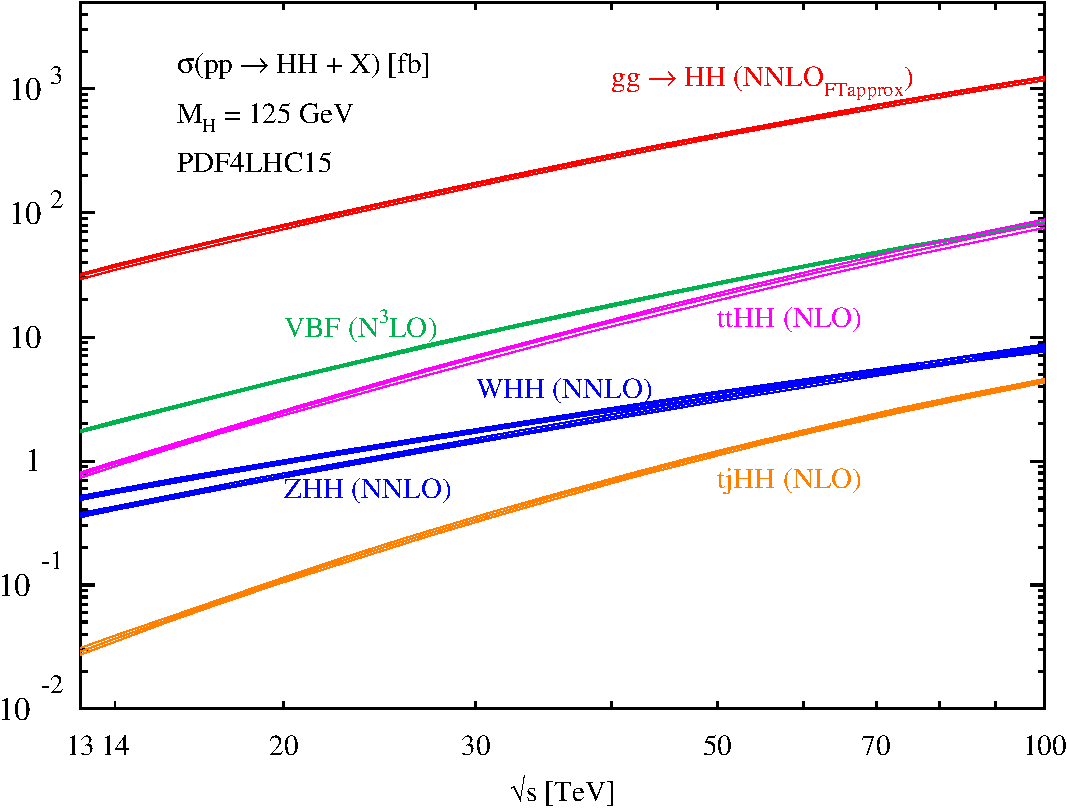
\includegraphics[width=0.85\textwidth]{Images/Theory/cxn_HH.pdf}
    \caption{Higgs pair production cross sections for different production modes, as a function of center of mass energy.}
    \label{fig:ProductionModeXSs}
\end{figure}

For proton-proton collisions at center-of-mass energies between 13-100 TeV, the dominant production mode of Higgs pair production is gluon-gluon fusion. For most of this energy spectrum, the next most sensitive production mode is Vector Boson fusion, roughly a factor of 20 less likely. Theoretical productions of Higgs pair production cross section, and physics processes in general, are extremely important for motivating the types of particle colliders and detectors to be built in the future. This allows the matching of a desired physics program with colliders and experiments expected to be capable of producing and detecting these expected physics signatures, in order to answer physicists' questions. 